\documentclass[a4paper,12pt,oneside]{book}

%-------------------------------Start of the Preable------------------------------------------------
\usepackage[english]{babel}
\usepackage{comment}
\usepackage{blindtext}
%packagr for hyperlinks
\usepackage{hyperref}
\hypersetup{
	colorlinks=true,
	linkcolor=blue,
	filecolor=magenta,      
	urlcolor=cyan,
}

\urlstyle{same}
%use of package fancy header
\usepackage{fancyhdr}
\setlength\headheight{26pt}
\fancyhf{}
%\rhead{
\includegraphics[width=1cm]{logo}}
\lhead{\rightmark}
\rhead{
\includegraphics[width=1cm]{logo}}
\fancyfoot[RE, RO]{\thepage}
\fancyfoot[CE, CO]{\href{http://www.e-yantra.org}{www.e-yantra.org}}

\pagestyle{fancy}

%use of package for section title formatting
\usepackage{titlesec}
\titleformat{\chapter}
{\Large\bfseries} % format
{}                % label
{0pt}             % sep
{\huge}           % before-code

%use of package tcolorbox for colorful textbox
\usepackage[most]{tcolorbox}
\tcbset{colback=cyan!5!white,colframe=cyan!75!black,halign title = flush center}

\newtcolorbox{mybox}[1]{colback=cyan!5!white,
	colframe=cyan!75!black,fonttitle=\bfseries,
	title=\textbf{\Large{#1}}}

%use of package marginnote for notes in margin
\usepackage{marginnote}

%use of packgage watermark for pages
%\usepackage{draftwatermark}
%\SetWatermarkText{
\includegraphics{logo}}
\usepackage[scale=2,opacity=0.1,angle=0]{background}
\backgroundsetup{
	contents={
\includegraphics{logo}}
}

%use of newcommand for keywords color
\usepackage{xcolor}
\newcommand{\keyword}[1]{\textcolor{red}{\textbf{#1}}}

%package for inserting pictures
\usepackage{graphicx}

%package for highlighting
\usepackage{color,soul}

%new command for table
\newcommand{\head}[1]{\textnormal{\textbf{#1}}}


%----------------------End of the Preamble---------------------------------------


\begin{document}
	
	%---------------------Title Page------------------------------------------------
	\begin{titlepage}
		\raggedright
		{\Large eYSIP2017\\[1cm]}
		{\Huge\scshape Fi-Pi Raspberry-Pi Adaptor Board for Firebird-V\\[.1in]}
		\vfill
		\begin{flushright}\textbf{Interns:-}
			{\large Milanpreet Singh \\}
			{\large Tejaswini A \\}\textbf{Mentors:-}
			{\large Rutuja Ekatpure \\}
			{\large Deepa Avudiappan \\}
			{\large Duration of Internship: $ 22/05/2017-07/07/2017 $ \\}
		\end{flushright}
		
		{\itshape 2017, e-Yantra Publication}
	\end{titlepage}
	%-------------------------------------------------------------------------------
	
	\chapter[Project Tag]{Fi-Pi Raspberry-Pi Adaptor Board for Firebird-V}
	\section*{Abstract}
	The project aims at developing Raspberry-pi based Adaptor board for Firebird series Robots.As Raspberry- Pi can cater to more applications specifically in domain of image processing and IOT  and provides a new feature of onboard computing which was not present in earlier versions Firebird series.
	\\Main features included in this Raspberry- pi based firebird are :-\\
	\begin{itemize}
		\item Differnet communication choices i.e through XBEE,Bluetooth,USB,DB9, or any serial communication protocol of your choice can used for communication purposes.
		\item Interfacing Camera on board and live image capturing and video streaming enhances its capabilities and horizon of its applications in different domains.
	\end{itemize}
	\newpage
	\subsection*{Completion status}
	The work flow of the project designed and its completion status is as follows:-\\
	
	\begin{table}
		\centering
	\end{table}
	\begin{tabular}{ |p{4cm}|p{3cm}|p{6cm}|}
		\hline
		\textbf{Task} &  \textbf{Completion Status} &  \textbf{Remarks}\\
		\hline
		Understanding Firebird and Raspberry-Pi& Completed & Firebird and Raspberry -pi were studied and pins of firebird mapped properly and BAsic operations of Raspberry -Pi werev studied\\
		\hline
		Interfacing ADC and port Expander&Completed&ADC MCP3008 and Port Expander MCP23017 were interfaced with raspberry-pi and firebird by enabling spi and i2c communication and installing packages serial and smbus \\
		\hline
		Powering circuit for pi&Completed&A circuit for powering Raspberry-pi using LM7805BT with 3A current capacity was designed\\
		\hline
		Communication protocols&Completed& Communication protocols like XBEE,DB9,USB were tested by sending commands to firebird through pi\\
		\hline
		LCD and Motion control&Completed & LCD in 4 bit mode was interfaced using pi and motors were operated at different speeds\\
		\hline
		Camera interfacing&Completed & Camera was interfaced with pi and images, videos were saved on pi.\\
		\hline
		Adaptor Board PCB& Completed and revised to new version&PCB was designed and tested with firebird.A newer version was designed with some changes \\
		\hline
		Manual &Completed&Both Hardware and Software manuals were designed incuding all the features ob board with their codes .\\
		\hline
	\end{tabular}
	
\section{Hardware parts}
\begin{itemize}
	\item List of hardware 
	\begin{enumerate}
		\item Raspberry Pi \\
		\href{https://www.raspberrypi.org/documentation/.../RPI-CM-DATASHEET-V1_0.pdf
		} {Download Datasheet ,}
		\href{http://www.amazon.in/Raspberry-Pi-Model-1GB-Complete/dp/B00T2U7R7I} {Vendor Details}
		\begin{figure}[h]
			\hspace{4cm}
			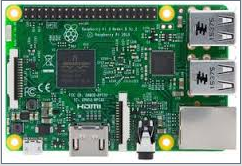
\includegraphics[width=0.3\textwidth]{RPi}
			\caption{ Raspberry Pi}
		\end{figure}
	\item FireBird V Robot \\
	\href{www.nex-robotics.com/fire-bird-v-atmega2560/fire-bird-v-atmega2560.html} {Download Datasheet ,}
	\href{http://www.nex-robotics.com/products/fire-bird-v-robots/fire-bird-v-atmega2560-robotic-research-platform.html} {Vendor Details}
\begin{figure}[h]
	\hspace{4cm}
	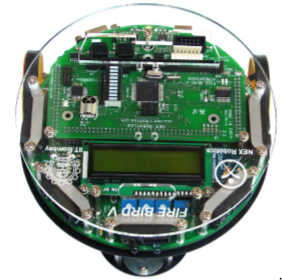
\includegraphics[width=0.3\textwidth]{robot}
	\caption{FireBird V Robot}
\end{figure}
	\item MCP23017 IC     \\
	\href{ww1.microchip.com/downloads/en/DeviceDoc/21952b.pdf
	} {Download Datasheet ,}
	\href{http://www.smddevices.com/} {Vendor Details}
		\begin{figure}[h]
		\hspace{4cm}
		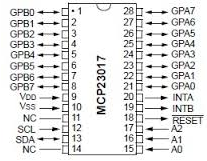
\includegraphics[width=0.3\textwidth]{mcp23017}
		\caption{ MCP23017 IC }
	\end{figure}
 \item MCP3008 IC       \\
\href{https://cdn-shop.adafruit.com/datasheets/MCP3008.pdf} {Download Datasheet ,}
\href{http://www.dnatechindia.com/MCP3008-10-Bit-ADC.html} {Vendor Details}
\begin{figure}[h]
	\hspace{4cm}
	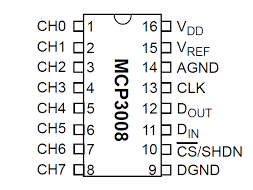
\includegraphics[width=0.3\textwidth]{mcp3008}
	\caption{ MCP3008 IC }
\end{figure}
\item FT232 IC       \\
\href{www.ftdichip.com/Documents/DataSheets/ICs/DS_FT232R.pdf
} {Download Datasheet ,}
\href{http://www.dnatechindia.com/ft-232-usb-uart-ic.html} {Vendor Details}
\begin{figure}[h]
	\hspace{4cm}
	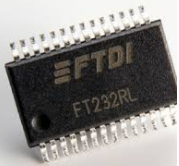
\includegraphics[width=0.3\textwidth]{ft232}
	\caption{ FT232 IC }
\end{figure}
\item MAX202 IC       \\
\href{www.ti.com/lit/ds/symlink/max202.pdf
} {Download Datasheet ,}
\href{https://www.tanotis.com/products/tanotis-2pcs-maxim-integrated-products-max202-max202ese-max202ese} {Vendor Details}
\begin{figure}[h]
	\hspace{4cm}
	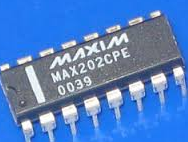
\includegraphics[width=0.3\textwidth]{max202}
	\caption{ MAX202 IC }
\end{figure}
\item LM324 IC       \\
\href{www.ti.com/lit/ds/symlink/lm124-n.pdf
} {Download Datasheet ,}
\href{http://www.dnatechindia.com/LM324.html} {Vendor Details}
\begin{figure}[!ht]
	\hspace{4cm}
	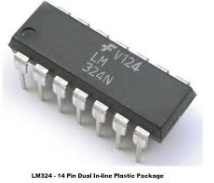
\includegraphics[width=0.3\textwidth]{lm324}
	\caption{LM324 IC }
\end{figure}
\pagebreak
\item LM7805 IC       \\
\href{https://www.sparkfun.com/datasheets/Components/LM7805.pdf
} {Download Datasheet ,}
\href{http://www.dnatechindia.com/LM7805.html} {Vendor Details}
\begin{figure}[!ht]
	\hspace{4cm}
	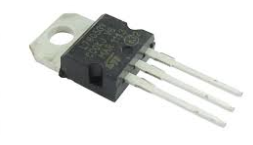
\includegraphics[width=0.3\textwidth]{7805}
	\caption{LM7805 IC }
\end{figure}
\item LM1117 IC       \\
\href{www.ti.com/lit/ds/symlink/lm1117.pdf
} {Download Datasheet ,}
\href{http://www.dnatechindia.com/lm-1117-1-8-v-smd-voltage-regulator.html} {Vendor Details}
\href{http://www.dnatechindia.com/LM7805.html} {Vendor Details}
\begin{figure}[!ht]
	\hspace{4cm}
	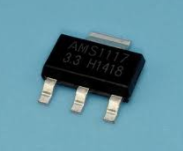
\includegraphics[width=0.3\textwidth]{1117}
	\caption{LM1117 IC }
\end{figure}
\item LED
\item Resistor
\item Bargraph LED
\item Switches
\item Header pins
\pagebreak

	
	\end{enumerate}
	\end{itemize}
	
	\section{Software used}
	\begin{itemize}
		\item MobaXterm  
		\href{http://mobaxterm.mobatek.net/MobaXterm_Setup_9.4.msi} {Download Link}\\
		Personal Edition 9.4
		\item Raspbian Jessie   
		\href{https://downloads.raspberrypi.org/raspbian_latest}{Download Link}\\
		Disk Image Version 2
		\item Autodesk Eagle 
		\href{http://www.cadsoftusa.com/download-eagle/}{Download Link}\\
		Version 8.2.1 
		\item XCTU 
		\href{http://www.digi.com/products/xbee-rf-solutions/xctu-software/xctu#productsupport-utilities}{Download Link}
		\item Win32 Disk Imager
		\href{http://sourceforge.net/projects/win32diskimager/}{Download Link}
		\item SD card Formatter
		\href{https://www.sdcard.org/downloads/formatter_4/eula_windows/}{Download Link}
		\item DHCP server
		\href{http://www.dhcpserver.de/cms/release_notes/2-5-2/}{Download Link}\\
		Version 2.5.2
		\item Serial Terminal 
		\href{https://serial-port-terminal.en.softonic.com/}{Download Link}
	\end{itemize}
	
	\section{Assembly of hardware}
	\subsection*{Circuit Diagram}
	\begin{figure}[!ht]
		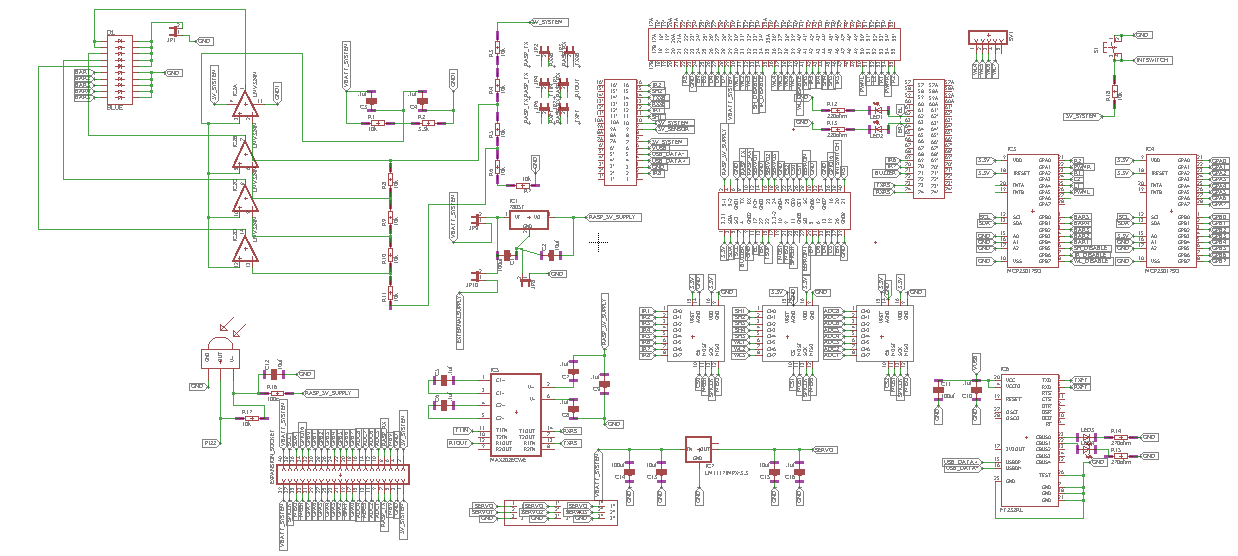
\includegraphics[width=1.1\textwidth]{schematic}
		\caption{schematic }
	\end{figure}
For more details refer to github link \href{https://github.com/eYSIP-2017/eYSIP-2017_Fi_Pi/blob/master/Documents/PCB_Schematics/Fi-Pi.sch} {Fi-Pi schematics}
	\pagebreak
	\subsection*{Eagle Layout}
\begin{figure}[!ht]
	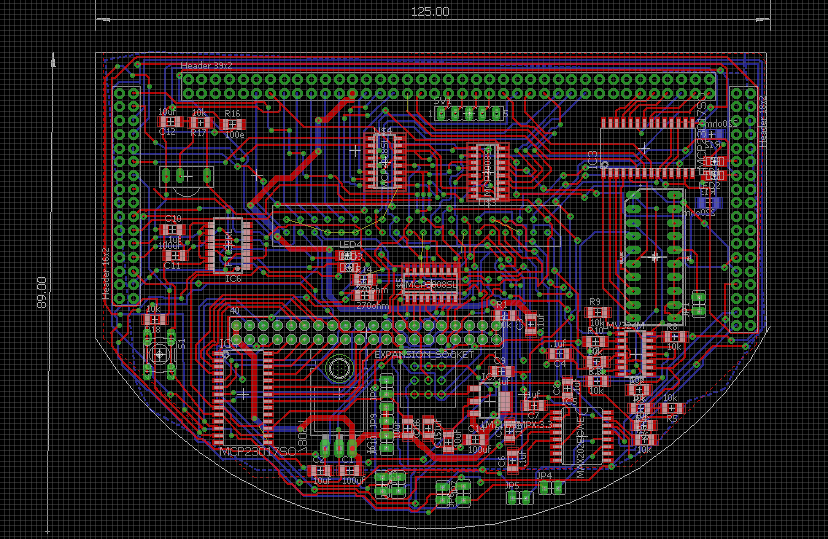
\includegraphics[width=1.1\textwidth]{layout}
	\caption{PCB board layout }
\end{figure}
For more details refer to github link \href{https://github.com/eYSIP-2017/eYSIP-2017_Fi_Pi/blob/master/Documents/PCB_Schematics/Fi-Pi.brd} {Fi-Pi layout}
\section*{Steps for Assembling the parts}
\subsection*{Step 1}
Get the PCB etched with the gerber file created from the eagle board layout. 
\pagebreak
\begin{figure}[!ht]
	\hspace{3cm}
	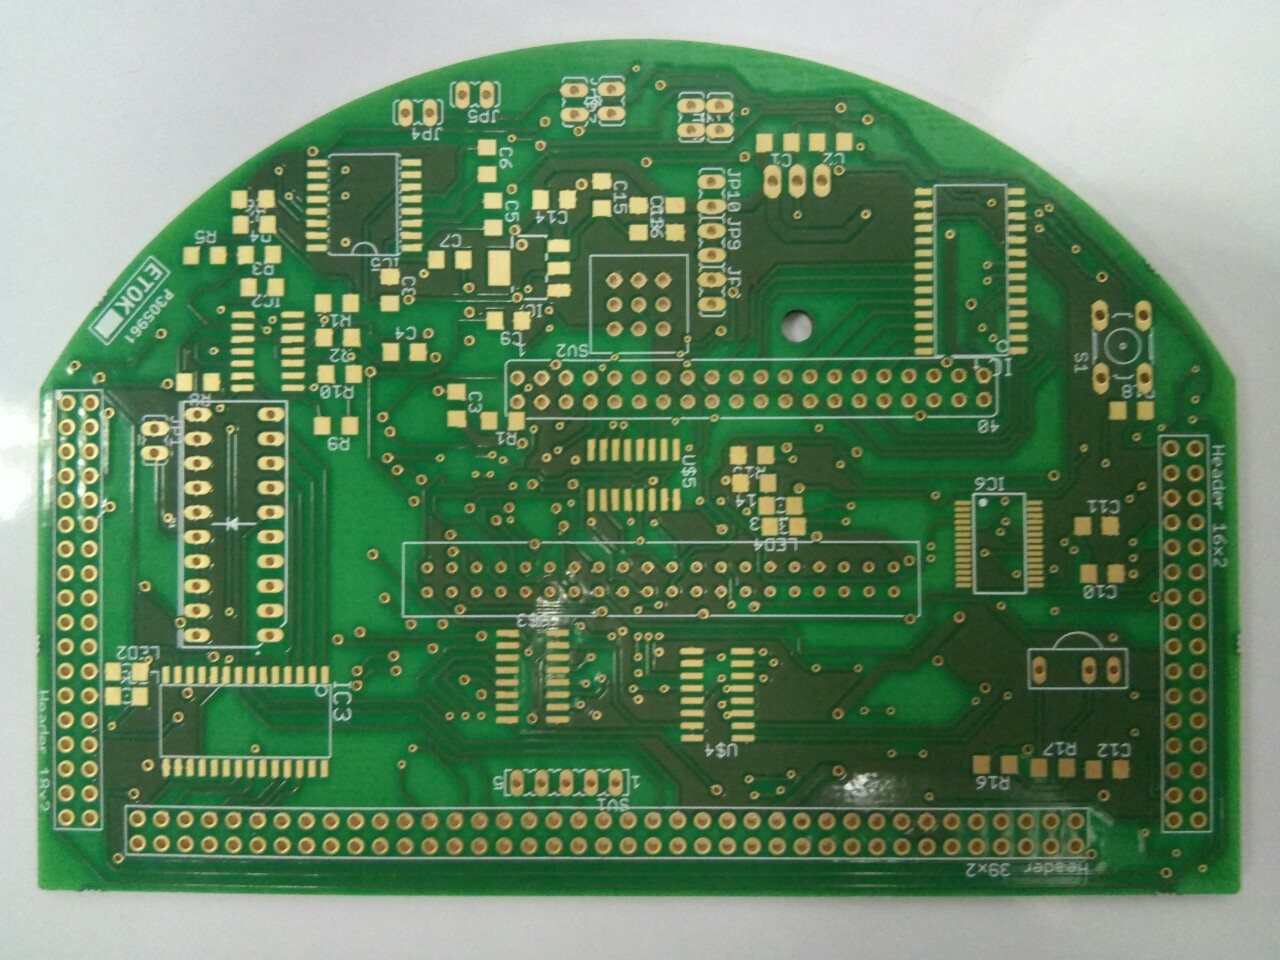
\includegraphics[width=0.6\textwidth]{solder_pcb}
	\caption{PCB board layout }
\end{figure}
\subsection*{Step 2}
Place the SMD and Through hole components appropriately in proper orientation and location. Finally solder them
\begin{figure}[!ht]
	\hspace{3cm}
	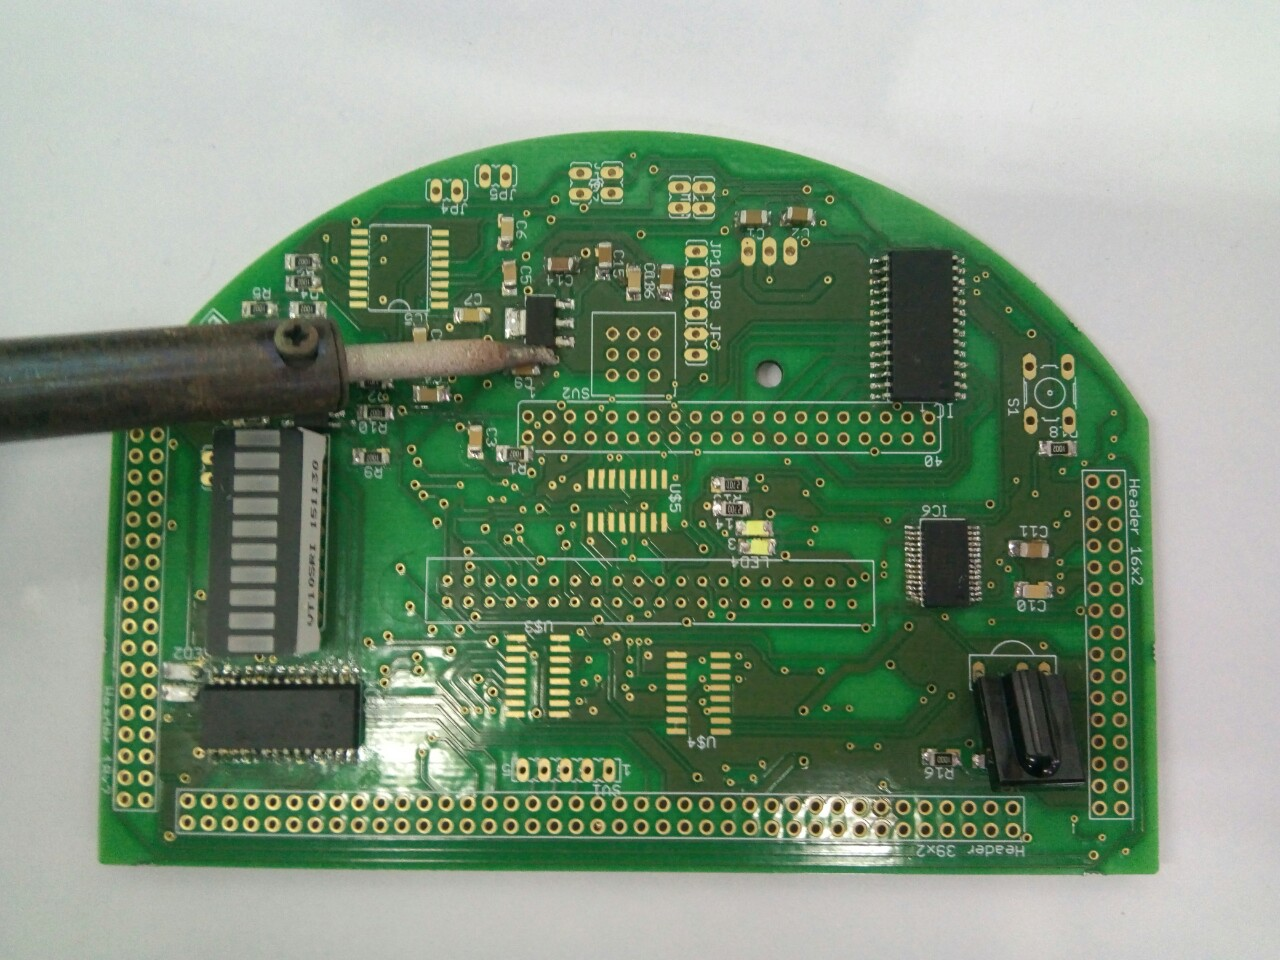
\includegraphics[width=0.6\textwidth]{plain_pcb}
	\caption{PCB board layout }
\end{figure}
\subsection*{Step 3}
The final PCB looks as shown below.
\begin{figure}[!ht]
	\hspace{3cm}
	\includegraphics[width=0.6\textwidth]{PCB}
	\caption{PCB board layout }
\end{figure}
	
	\section{Software and Code}
	\href{https://github.com/eYSIP-2017/eYSIP-2017_Fi_Pi/tree/master/codes/Experiments}{Github link} for the repository of code

	\section{Future Work}
	Raspberry-pi is a good option for IOT applications so a website can be designed which could be linked to the Raspberry-pi enabled Firebird and data from firebird can be regularly sent let be the sensor values and displayed on the site and stored for further applications.\\
	It may help in tracking conditions of environment from internet and making plant watering bot by detecting plants in the garden through image processing and water them by detecting the humidity and hence watering accordingly. 
	\pagebreak
	\section{Bug report and Challenges}
	Some changes in Hardware (PCB) have been made and a newer version of PCB is designed:-
	\begin{itemize}
		\item External powering port with external separate battery
		\item Raspberrypi pin header modified for plug and play directly
		\item Transistors are interfaced instead of jumpers for changing the communication platform from one to another and hence can be controlled through software means.
		\item Motors moved to Pi pin header and LCD to port expander beacuse LCD is somewhat useless as we can do ssh and check it on laptop and hence saving power.
	\end{itemize}
	
	\begin{thebibliography}{li}
		\bibitem{wavelan97}
		Raspbian Jessie OS Installation,
		{\em https://www.engadget.com/2012/09/04/raspberry-pi-getting-started-guide-how-to/}
		\bibitem{wavelan97}
		SPI and I2C communication protocol
		{\em www.byteparadigm.com/applications/introduction-to-i2c-and-spi-protocols/}
		\bibitem{wavelan97}
		I2C configuration
		{\em https://learn.adafruit.com/
			adafruits-raspberry-pi-lesson-4-gpio-setup/
			configuring-i2c}
		\bibitem{wavelan97}
		Pulse Width Modulation
		{\em http://www.electronics-tutorials.ws/blog/
			pulse-width-modulation.html}
		\bibitem{wavelan97}
		Software Interrupt
		{\em https://www.techopedia.com/denition/22195/software-interrupt}
		\bibitem{wavelan97}
		Port expander MCP23017 IC
		{\em https://www.mathworks.com/examples/matlab/4547-add-digital-i-o-pins-to-raspberry-pi-hardware-using-mcp23017}
		\bibitem{wavelan97}
		Queries regarding Raspberry Pi
		{\em http://stackoverflow.com/questions/tagged/raspberry-pi}
		\bibitem{wavelan97}
		Libraries for progrmming different IC's or modules
		{\em https://github.com/adafruit}
	\end{thebibliography}
	
\end{document}